%%=============================================================================
%% Methodologie
%%=============================================================================

\chapter{Practical demonstration with Qiskit}
\label{ch:practical}

For 2 decades now people have been receiving fully blown quantum mechanics courses where they are able to experiment with the thought of quantum experiments in a theoretical type of way, but never were truly interested parties able to perform their experiments in a free and fluid manner. QC is at a point where we are able to effectively experiment with the technology as a broader community. Platforms like Qiskit are excellent in their reach towards interested parties and are more than welcoming towards new developments that could aid the whole community in its research. The service is open source which truly pushes the whole movement of research out of this shroud of high costs and large enterprises. This will obviously influence other branches to follow in the same footsteps as to allow every party that is interested or has a passion to be able to participate in a costless and open manner. To remain objective and fair towards other companies outside of IBM, Google is also participating in the open source community with platforms like Cirq, \textcite{Cirq}. 

In the following part, we will lay out how any interested parties are able to perform their own executions on real devices and start applying what some of them have been learning theoretically for over 20 years. Whilst trying to resolve the main question of this specific paper `How will quantum computing affect the mainframe environment and its applications? `, a major roadblock has been discovered, which is interesting none the less because it shows were research and engineering has not yet ventured far enough to overcome them. 

So the question remains is there a practical example where we would be able to show how a quantum algorithm could be applied on the large quantity of mainframe data generated each day? And the answer at the time of writing would be that as of now it is not yet feasible to process large quantities of batch data. So for now we have chosen for an algorithm that could prove useful once implemented on a database structure inside the mainframe.

\subsection{Grover's search algorithm in a practical fashion}
\subsubsection{Grover's search unstructured database search}

We have chosen for an adaptation of an algorithm that could prove extremely useful for any implementation together with a mainframe, which is the Grover Search algorithm applied for the boolean satisfiability problem. The whole premise of the original algorithm is that we are able to speed up the search time in an unstructured database quadratically. This all meaning when a computer needs to find an item with an unique attribute that differentiates itself from the other items in the list, QC could become the main solution. The whole algorithm uses something called "amplitude amplification" where the algorithm influences the probabilities in such a manner that the specific item has the highest probability after the Quantum computation. \autocite{Grover1996}

To clarify amplitude amplification further, this is a principle that affects qubits in their superposition and entangled states where they would interfere with each other to eliminate the least likely outcomes and push up the statistical chance of the desired item. By applying this to an algorithm after the correct transformations, you would be able to decompose all the different results back to a highly probable result that does not collapse all the qubits in superposition like a normal measurement would. 

\subsubsection{Grover's search algorithm in an applied form}

For the experiment itself, we have chosen for the "Boolean satisfiability problem" which uses Grover's way of amplitude amplification to find the correct result. This computer science question goes as follows, given a boolean comparison of multiple parts are we able to determine the outcome to get that specific TRUE. Being able to solve this comparison in a single execution could abuse the fact of superposition and could prove useful when we scale out the problem towards thousands or even millions of comparisons for other algorithms. For now the 3-SAT problem has been chosen to be performed using Qiskit to show off the potential of QC for now.

You are able to view the function stated below as the problem that we will try and solve using Quantum technology. The algorithm now needs to find which solutions are possible by interchanging x,y,z with TRUE/FALSE.

$ f(x,y,z) = (\neg x \vee y \vee \neg z) \wedge  ( x \vee \neg y \vee \neg z) \wedge ( x \vee \neg y \vee  z) \wedge (\neg x \vee \neg y \vee z) \wedge  ( x \vee y \vee  z)	 $
				 
\subsubsection{Executing the quantum algorithm}				 

Using a simulator of an ideal quantum computer we are able to show the results in figure 4.1 below. The probabilities have been amplified to where they are the correct results of this boolean expression. Figure 4.2 shows the gathered results when we sent off the identical circuit towards one of IBM's real quantum devices (IBMQMelbourne16 in this case). 

\begin{figure}[h]
	\centering
	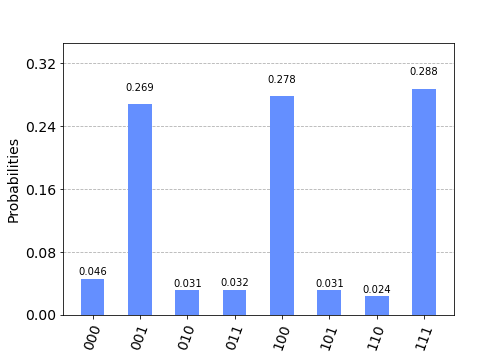
\includegraphics[scale = 0.75]{../Demonstration/img/simulated_3SAT.PNG}
	\caption{These are the results of executing the algorithm for the 3-SAT problem on a \textbf{quantum simulator} that comes with Qiskit. The encoding refers to the TRUE/FALSE value of the x,y,z respectively}
\end{figure}


\begin{figure}[h]
	\centering
	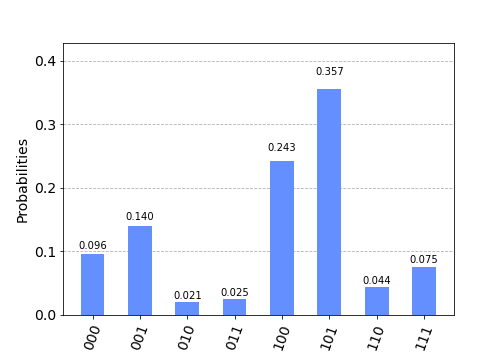
\includegraphics[scale = 0.75]{../Demonstration/img/real_device_3SAT.PNG}
	\caption{These are the results of executing the algorithm for the 3-SAT problem using 15 qubits on a \textbf{real quantum device} that comes with Qiskit. The encoding refers to the TRUE/FALSE value of the x,y,z respectively}
\end{figure}

The reason for choosing this specific experiment is to show that even problems that just require us to encode boolean statements we needed 694 quantum gates. IBMQ transpiles the sent-off circuit to the necessary amount of gates needed for this specific calculation. It does not keep in account that having this much gates on a single line of computation invites a multitude of quantum decoherence issues during runtime. 

If you have looked closely at the image above (figure 4.2) you are able to see that decoherence for now breaks the probabilities of a computation too much to reliably trust any computation of this size out of a quantum computer. The values become distorted over time by all types of interference even if all the interference from inside the machine is not accounted for the machine can become influenced by a single external interaction like temperature, pressure etc. 

\begin{center}
	\begin{tabular}{|| c c ||}
		\hline
		$f(x,y,z)$ & TRUE/FALSE \\
		\hline\hline
		0 0 0 & FALSE \\ 
		0 0 1 & TRUE \\
		0 1 0 & FALSE \\
		0 1 1 & FALSE \\
		1 0 0 & TRUE \\
		1 0 1 & FALSE \\
		1 1 0 & FALSE \\
		1 1 1 & TRUE \\
		\hline
	\end{tabular}
\end{center}

If we compare the manually gathered results in the table above across the simulated version and the real version, we are clearly able to see that decoherence has played too big of a role to be certain of any reliable output for these types of large computations. By having these big differences in results we once again prove that simply adding qubits will not be helpful for the reliability in QC. The results differ too much to ever use these results in business cases where speed is as critical as accuracy in reporting towards externals.
Let us work out a clear example to make sure our probabilities generated by the real quantum device are incorrect. If we take the highest probability of the real execution which is the configuration of $101$. Meaning that the quantum computer determined that when X and Z are true the whole boolean expression will result in a returned value of TRUE. This is simply not a valid option for this boolean expression. If we look at the first part of this boolean expression we can see that this configuration would return a FALSE resulting in the whole expression being FALSE because all the parts are connected with a logical AND. 

$f(1,0,1) = (0 \vee 0 \vee 0 \vee) \wedge (1 \vee 1 \vee 0)  \wedge ( 1 \vee 1 \vee  1) \wedge ( 0 \vee 1 \vee 1) \wedge  ( 1 \vee 0 \vee  1)$


\subsection{Data-encoding in QC}

As the experiment clearly shows there is an actual advantage reachable with quantum computing. Of course quantum decoherence is a main aspect of QC and solving it would be greatly beneficial for the whole sector, but there is also a different problem that arises with defining our classical way of problems in a quantum way. The way we represent data in a quantum circuit quickly becomes overly complicated for any large database structure.

For now quantum computers are great in predicting what quantum effects will occur and where quantum physics influences specific sectors. And by using them for use-cases like simulating quantum effects we can already see the advantages to the businesses itself. The issue lies in the fact that we want to input  classical database structures into a quantum device and hopefully receive the results in a readable classical solution. 

This shows an issue we are facing with the encoding of our classical data to quantum data and back. For the proof-of-concept experiments it does not matter as the encoding time really does not influence the experiment as a whole. But once we start scaling out the issue where we would want to find a specific item through the use of Grover's algorithm, we would run into the issue that the encoding and decoding of the input and output could take up a great amount of computational time. If however QC develops in such a way that we are able to gain the full benefits of qubits in superposition this encoding time could be overcome, but for now it remains a crucial factor in solving the whole feasibility of QC.



\subsection{Mainframe computing with QC}

As the paper has previously stated having QC together with the power of a mainframe could become extremely advantageous for the whole industry to provide the power of data crunching this immense layer of internal data that companies have collected over the years. So we needed to find a circuit that could show of where quantum computing indeed could benefit in the crunching of data in a better/ faster way than classical computing can at the moment. Soon it became clear that simulating anything of a mainframe is impossible for now, we can simulate how a new form of database search could work with Grover. But we are not able to simulate the main advantage of a mainframe device, which is performing quick, stable and secure input and output transformations. And as shown by the experiment it is obvious that having a stable output of a specific input is not one of the main strengths of QC. Then when we take into account the encoding and decoding of classical computations and problems, which would greatly slow down the performance of a mainframe.

So for now there is no clear advantage when we use the current developments of QC with the existing mainframe technology. It does not take away its immense potential when QC is able to process the complete I/O of a mainframe in an exponentially smaller time frame than classical computing processing is able to do now.

Then obviously there remains the issue that quantum processors don't have the capability to actually perform algorithms that require a greater amount of qubits due to decoherence and previously stated problems.

\subsubsection{Future prospects}

As for now we are able to play around with the greater problems of quantum computing but to be able to \underline{reliably} solve real-world solutions in a beneficial way remains an uncertainty.

So with the current state of engineering, computer scientists will have to wait to fully utilise the system in a reliable fashion. But as engineering develops the power of quantum computing will increase exponentially with each added qubit to the system, which would make algorithms like this extremely valuable for data-crunching. When we find a way to circumvent the interference of quantum decoherence or when we reliably fix the errors it produces, a quantum system could become an essential tool for every sector willing to innovate. 


